\subsection{Train Custom Data: Weights, Biases Logging, Local Logging}

As shown in Figure~\ref{fig:colab_metrics}, the average accuracy, precision, and recall of the model all show a significant increase with the model training number when the Intersection Over Union (IOU)\footnote{IOU is an evaluation metric used to measure the accuracy of an object detector on a particular dataset.} is between 50\% and 95\%. In particular, the precision of the model can eventually reach a level close to 96\%. However, this does not necessarily mean that the model will also fit the satellite imagery of the Gulf of California. First, such high accuracy results only tell us that the model can achieve a relatively high recognition accuracy, which gradually increases and reaches 96\% after 300 training repetitions. In the case that the algorithm needs to be trained for this area, consideration must be given to purposefully selecting many small boats in or near the area as a data source for training the model. 

\begin{figure}[!t]
    \centerline{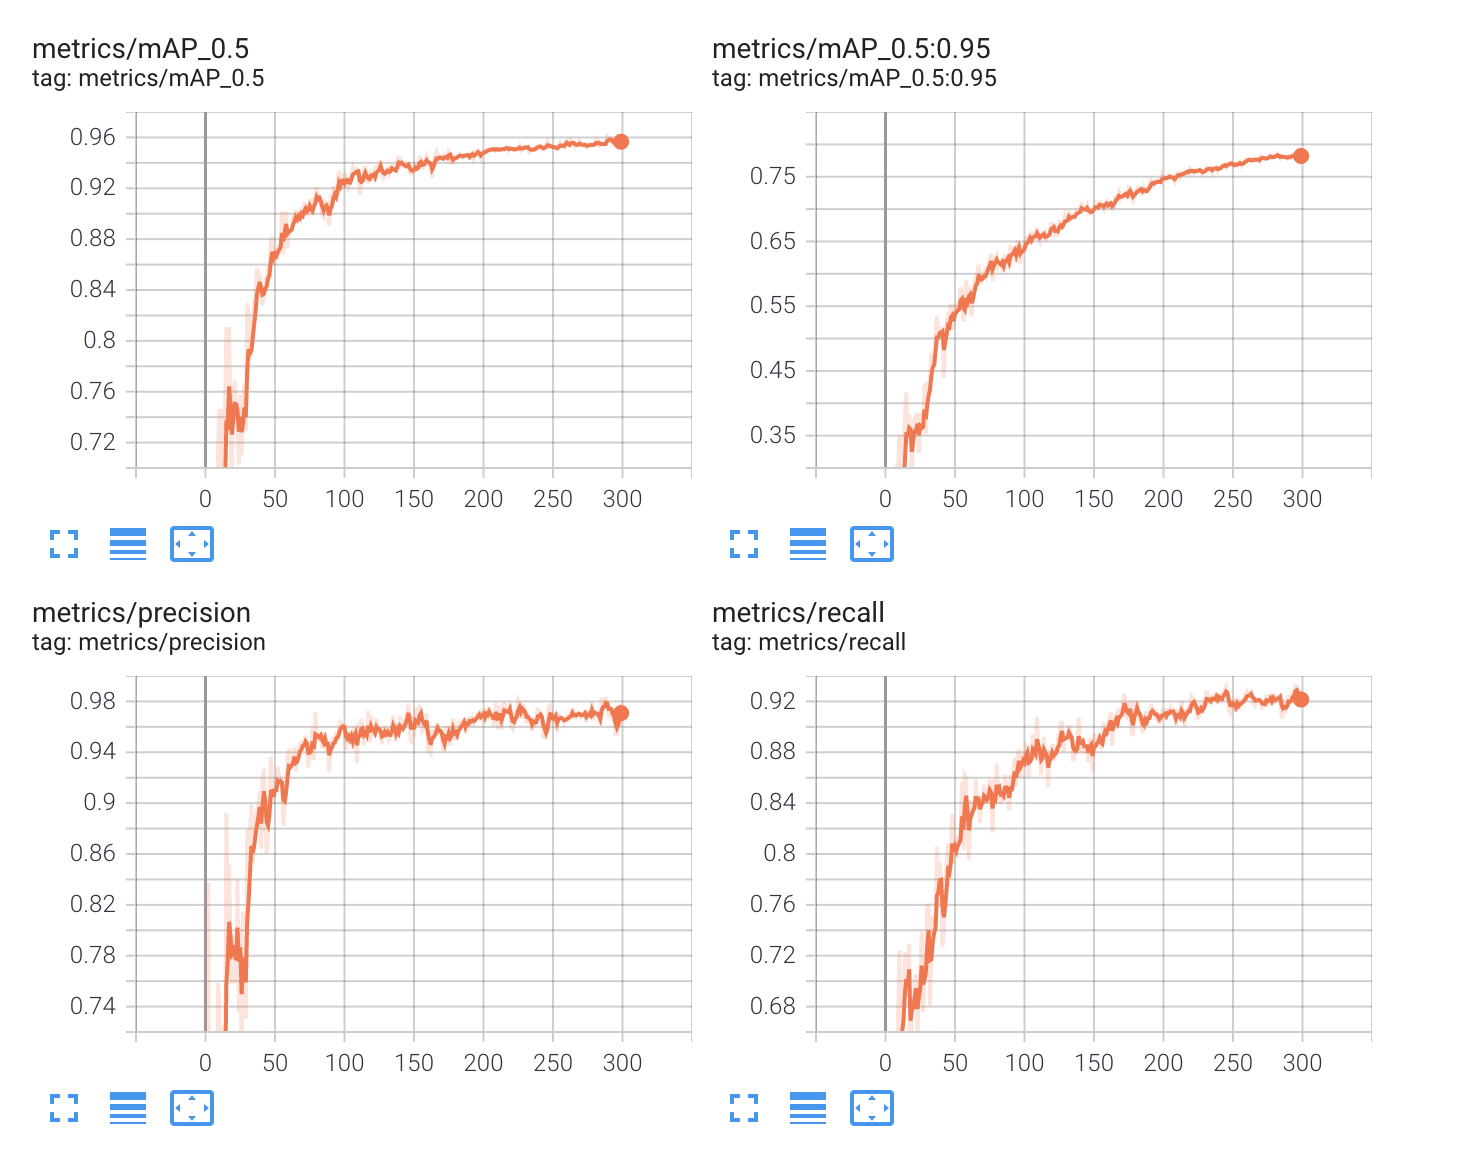
\includegraphics[width=\columnwidth]{img/colab_metrics.png}}
    \caption{Average model precision when IOU is larger than 0.5; Average model precision when IOU is between 0.5 and 0.95; The model precision; The model recall rate.}
    \label{fig:colab_metrics}
\end{figure}

To train models faster, we reduced the images' resolution by about 70, resulting in images of 416 pixels x 416 pixels. The training could otherwise take two weeks if the images used had a resolution of 4800 pixels x 2908 pixels.

Similarly, as shown in Figure~\ref{fig:colab_train}, the loss rate of the box can eventually reach 1\% as the number of training sessions increases. Since this study has defined only one class of object (i.e. boat), the probability that the detection box does not detect that it is a boat at all is 1\%. Similarly, because there is only one class, the class loss rate is 0. Figure~\ref{fig:test_batch1_pred} presents the prediction results during the training of the model, and shows that the model can detect the presence of vessels in 100\% of the tested ranges and gives the corresponding range boxes. Most detected boats have a 90\% probability of being boats, an acceptable value for object detection. Since only one class was set, some were also considered a 100\% probability of being boats.


\begin{figure}[!t]
    \centerline{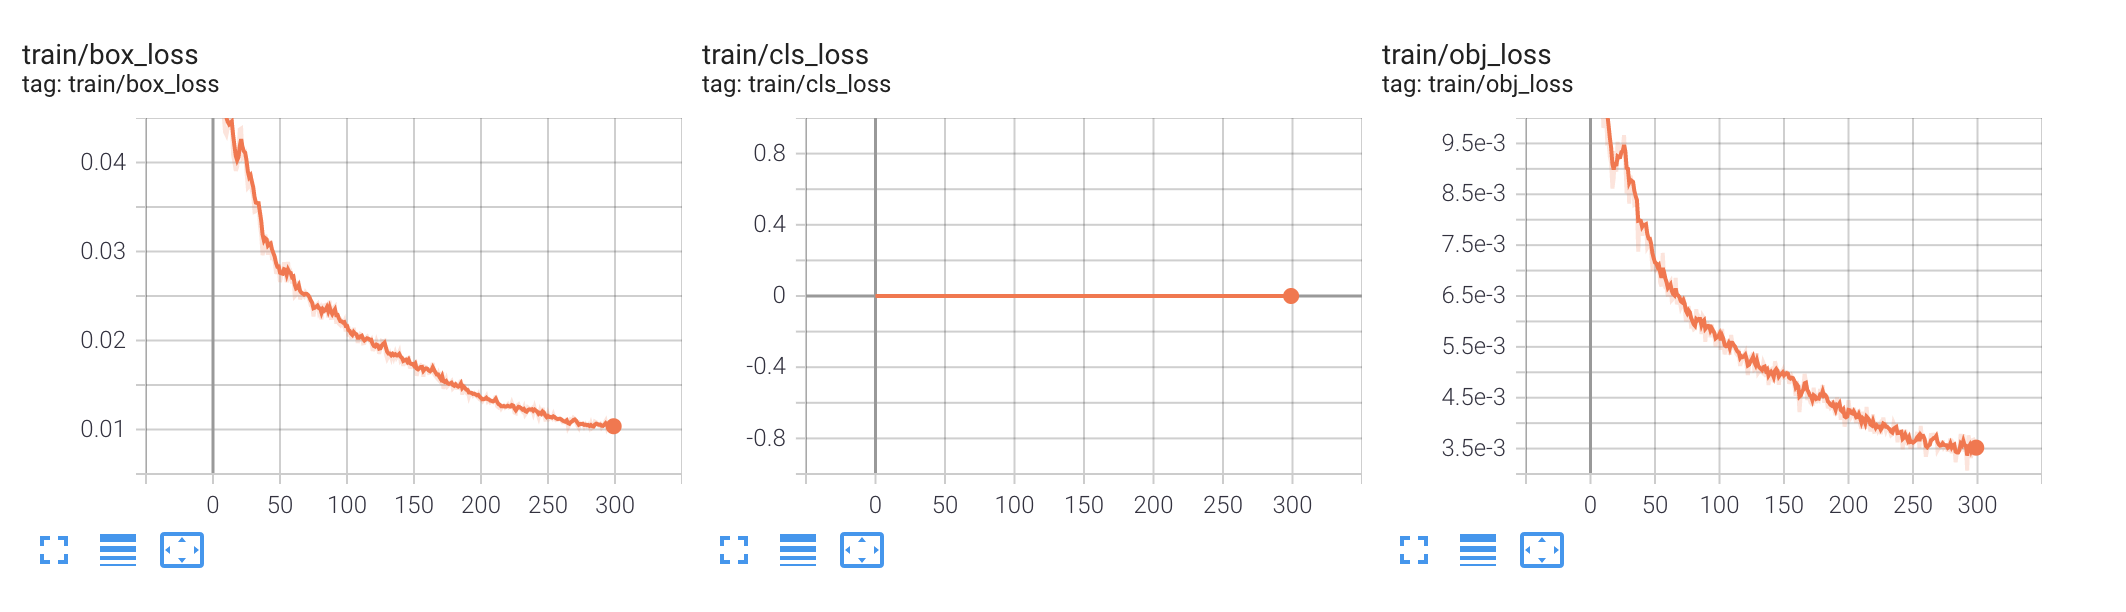
\includegraphics[width=\columnwidth]{img/colab_train.png}}
    \caption{The box loss rate of the model; The class loss rate of the model; The object loss rate of the model.}
    \label{fig:colab_train}
\end{figure}

\begin{figure}[!t]
    \centerline{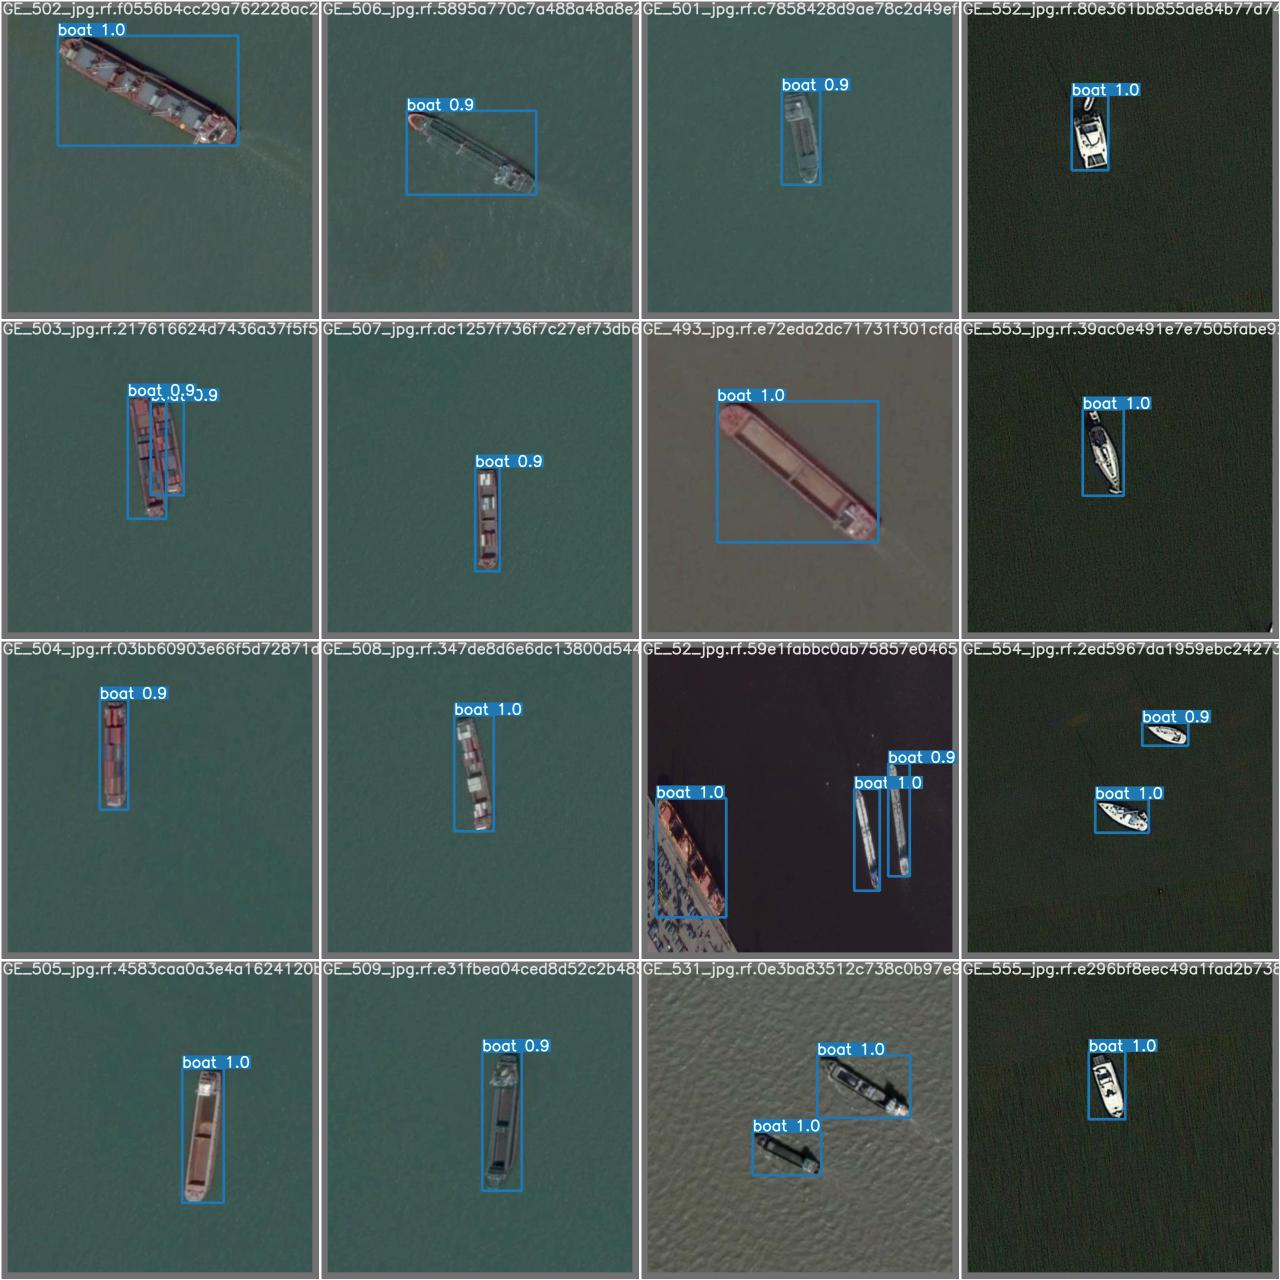
\includegraphics[width=\columnwidth]{img/test_batch1_pred.jpeg}}
    \caption{Test result of a trained model for detecting ships.}
    \label{fig:test_batch1_pred}
\end{figure}

\subsection{Detection Results and Small Boat Composition}
Starting with the length measurement comparison of a detected small boat and a large ship by BoatNet against Google Earth Pro measuring tools, Figure~\ref{fig:length_test} shows that the small boat detected measured 6.98 metres using Google Earth Pro, while BoatNet estimated 6.74 metres. The error between them is 3.4\%. Google Earth Pro measured the larger ship at 41.38 metres and BoatNet at 40.98 metres. The error between them is less than 1.0\%.

\begin{figure}[t]
    \center
    \includegraphics[width=\columnwidth]{img/length_test.png}
    \caption{Compare the length of boats using Google Earth ruler and computer vision algorithm. This example shows the image from Google Earth Pro for Zurich Lake on 16th August 2018 when the eye alt was 200 metres.}
    \label{fig:length_test}
\end{figure}

As explained in Sec~\ref{III-D-Detection-Architecture}, it was unproductive for the model to select the entire region for the study due to the varying amount of publicly available regional images from Google Earth Pro over the past three years. Ultimately, the satellite image database was built from 690 images. However, as stated in Sec~\ref{III-D-Detection-Architecture}, some of the slightly earlier satellite images offered inferior detail representation capabilities, which resulted in the model not accurately detecting the target's features. To improve model accuracy, an image enhancement process using a 5x5 sharpening kernel allowed for a higher recognition rate. However, the following situations still occur:

\begin{enumerate}
    \item Figure~\ref{fig:1_docked_together_Guaymas_202001_20}: When the detailed representation of the image is indigent, i.e., the images are blurred, and two or three small boats are moored together, the model is very likely to recognise the boats as a whole. There are two reasons for this problem. First, the training data is primarily a 'fuzzy' data source. Thus, when two or three small boats are moored together, the model cannot easily detect the features of each small boat individually. In contrast, it may seem more reasonable to the model that the boats as a whole have the same features. The second reason is that most data sources are individual boats on the surface or boats docked close to each other. As the data sources do not fully consider the fuzzy nature of the detail needed to detect the object and the fact that they are too close together, the model naturally does not recognise such cases.

    
    \item Figure~\ref{fig:2_square_Guaymas_202001_01}: When a large cargo ship is moored, the ship appears as a 'rectangle' from the air, much like a long pier, and is sometimes undetectable because small vessels with a rectangular shape were not common at the time the data feed was compiled. This also applies to uncommon vessels such as battleships. This could be corrected if the model considered larger ships, but this was outside the scope of this work.

    \item Figure~\ref{fig:3_beach_SantaRosalia_202104_02}: The recognition rate was also significantly lower when the boats sometimes lay on the beach rather than floating on the water. This is because most of the training data are based on images in the water rather than boats on the beach.

\end{enumerate}

\begin{figure}[!t]
    \centering
    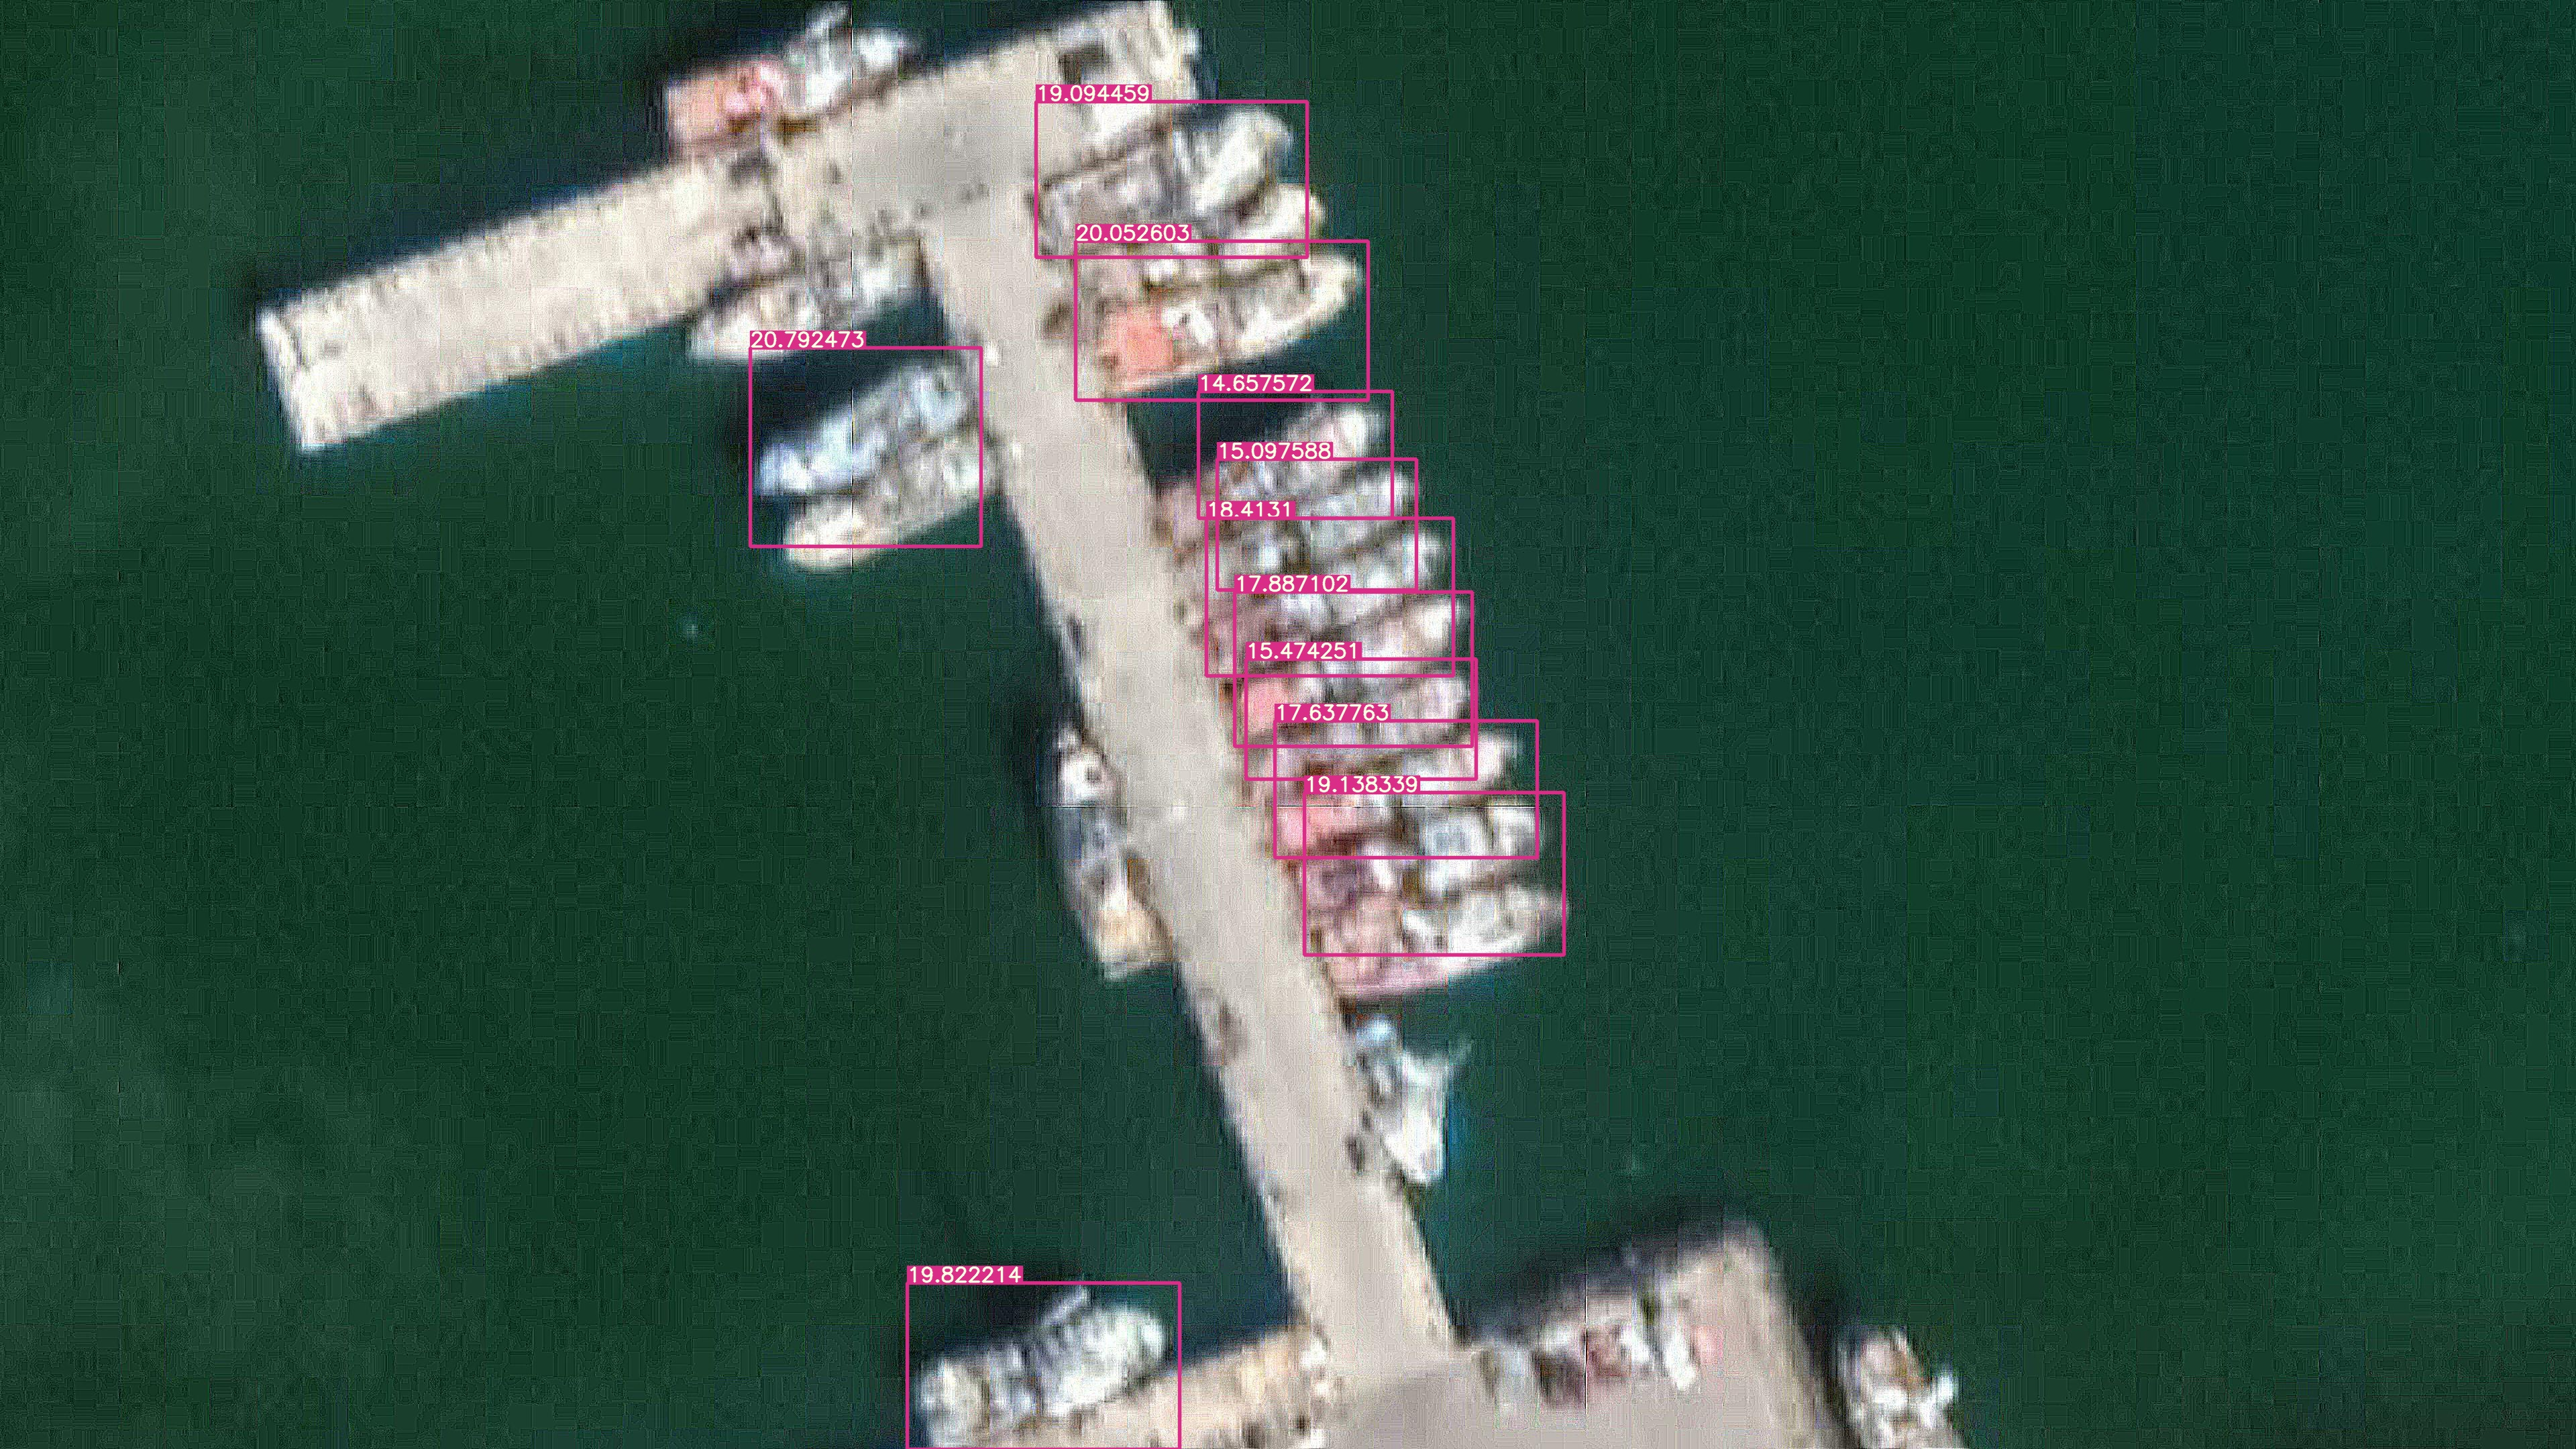
\includegraphics[width=\columnwidth]{img/1_docked_together_Guaymas_202001_20.jpeg}
    \caption{When small boats are moored closely together in the harbour, the model may recognise two small boats as one. The image is from Guaymas, January 2020.}
    \label{fig:1_docked_together_Guaymas_202001_20}
\end{figure}

\begin{figure}[!t]
    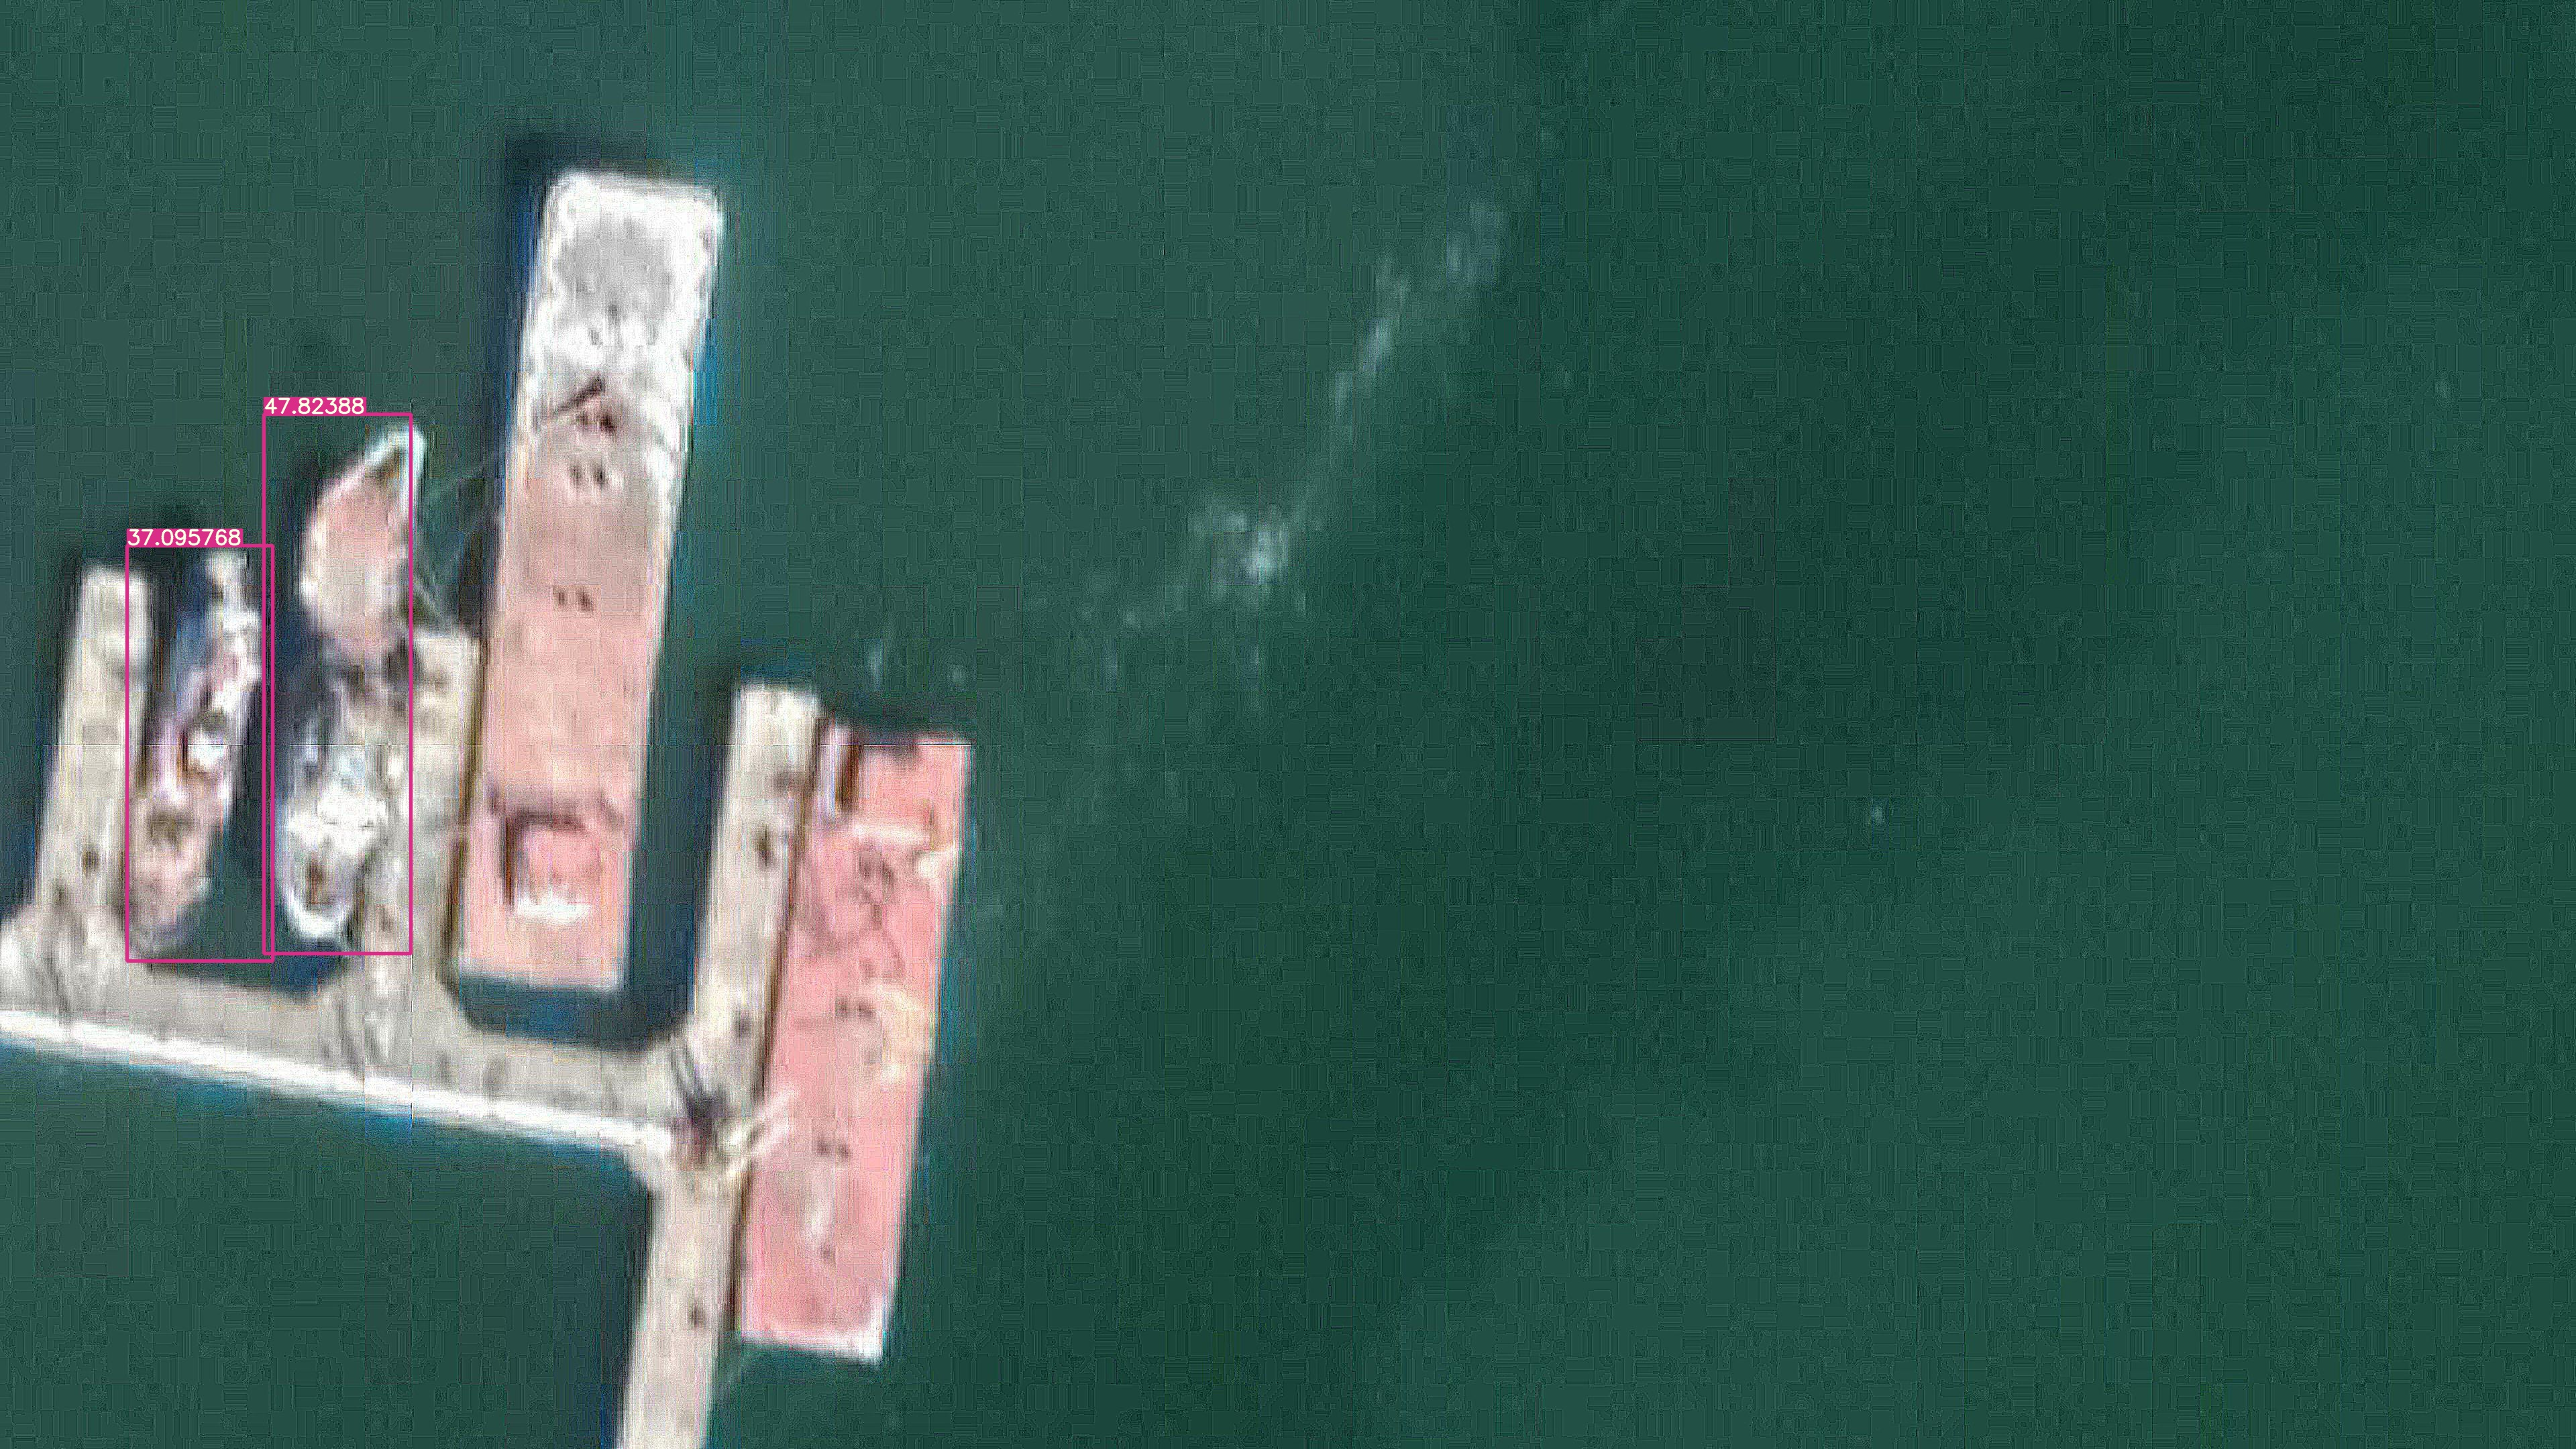
\includegraphics[width=\columnwidth]{img/2_square_Guaymas_202001_01.jpeg}
    \caption{When the cargo ship is full of cargo, the ship looks like a rectangular jetty from above and loses the normal shape of a ship. The image is from Guaymas, January 2020.}
    \label{fig:2_square_Guaymas_202001_01}
\end{figure}

\begin{figure}[!t]
    \includegraphics[width=\columnwidth]{img/3_beach_SantaRosalia_202104_02.jpeg}
    \caption{Models may have difficulty detecting small boats moored on the beach. The image is from Santa Rosalia, February 2021.}
    \label{fig:3_beach_SantaRosalia_202104_02}
\end{figure}



\begin{figure}[t]
    \center
    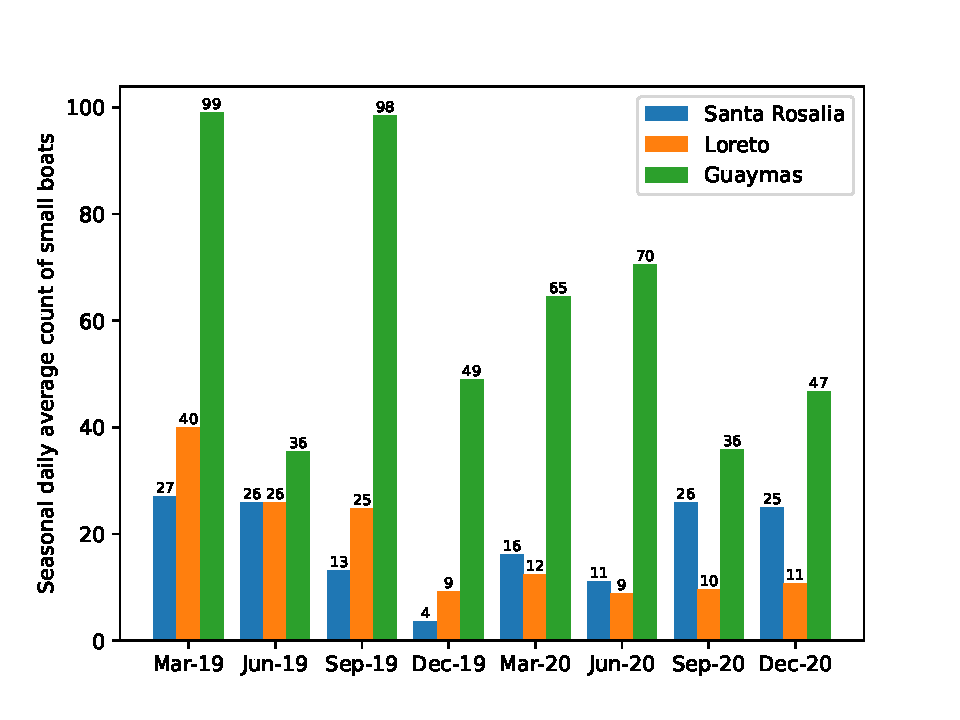
\includegraphics[width=\columnwidth]{img/avg_small.pdf}
    \caption{The seasonal daily average count of small boats in Santa Rosalia, Loreto, and Guaymas between 2019 and 2020.}
    \label{fig:avg_small}

    \center
    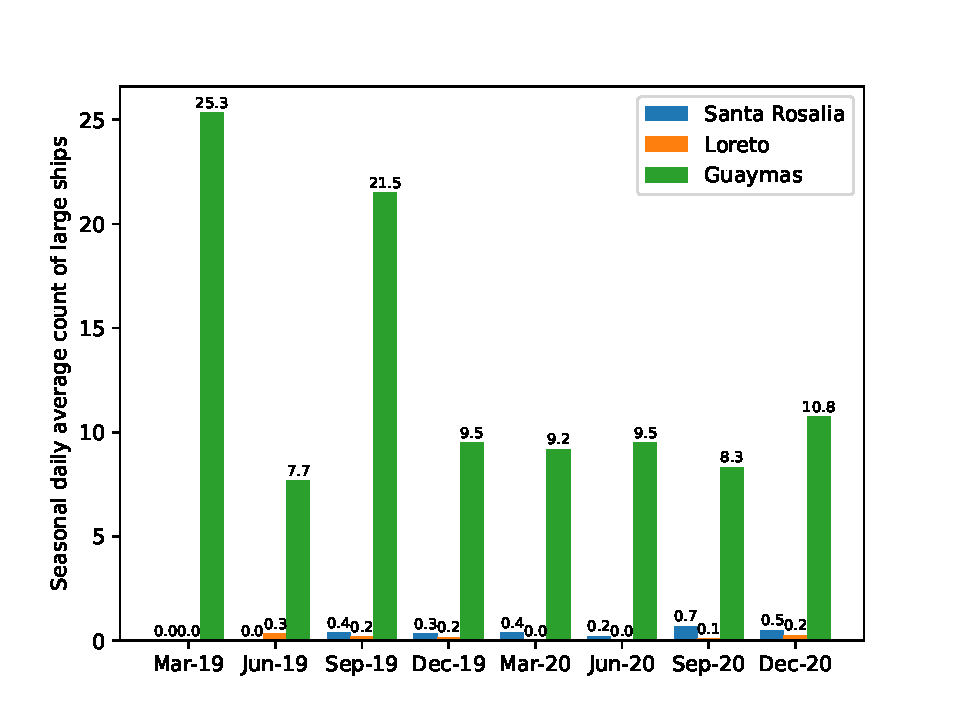
\includegraphics[width=\columnwidth]{img/avg_big.pdf}
    \caption{The seasonal daily average count of large ships in Santa Rosalia, Loreto, and Guaymas between 2019 and 2020.}
    \label{fig:avg_big}
\end{figure}

Nevertheless, as Figures~\ref{fig:1_docked_together_Guaymas_202001_20},~\ref{fig:2_square_Guaymas_202001_01},~\ref{fig:3_beach_SantaRosalia_202104_02} demonstrate, the model still detects most small boats in poorly detailed satellite images, even those that the human eye cannot easily detect. The number of small and large ships between regions can be seen in Figure~\ref{fig:avg_small} and Figure~\ref{fig:avg_big}. Two different types of port cities are exemplified by Guaymas, Loreto and Santa Rosalia:


\begin{enumerate}
    \item Santa Rosalia and Loreto have a much smaller number of small boats and almost no large ships.
    \item The port of Guaymas presented a larger number of small boats when contrasted to the other two coastal cities. There were between 1.37 and 8.00 times more small boats detected in Guaymas than in Santa Rosalia (dependent on the month and year of the image) and 3.00 times more than in Loreto. 
    \item Guaymas had a larger number of large ships as well. There were more than ten times more large ships detected in Guaymas than in Santa Rosalia and Loreto.
    \item In the relatively large seaports of Guaymas and Loreto, there is a tendency for both large and small vessels to decrease with time.
\end{enumerate}

In fact, according to statistic\cite{INEGI2022Population} from the Mexican government, in 2020, the populations of Guaymas, Loreto, and Santa Rosalia were 156,863, 18,052, and 14,357, respectively. Therefore, it seems that the number of detected boats is correlated to the number of habitats, which makes sense since, by probability, there would be more economical and leisure activities around larger coastal cities.


\subsection{Entertainment and Fishing Boats in the Gulf of California}



\begin{table}[t]
\center
\begin{tabular}{|c|c|c|c|c|}
\hline
                                &  Mar-20   & Jun-20    & Sep-20    & Dec-20\\ \hline
   Small boats                  &  323      & 283       & 215       & 187   \\ \hline
   Large ships                  &  46       & 38        & 50        & 43    \\ \hline
   Small white boats            &  302      & 273       & 210       & 174   \\ \hline
   Shipping boats               &  21       & 10        & 5         & 13    \\ \hline
\end{tabular}
\caption{\textbf{Detection example.} Small boats, large ships, and small white boats in Guaymas in 2020.}
\label{Guaymas_2020}
\end{table}

According to the statement in Sec~\ref{III-D-Detection-Architecture}, determining whether a boat is white can be used as a criterion to determine whether a boat is used for recreation or fishing. As seen in Table~\ref{Guaymas_2020}, most of the small boats captured in the photo of Guaymas in 2020 are white ( i.e. all can be classified as recreational boats). However, as previously discussed, this conclusion is limited since the algorithm does not consider, for example, other colours as part of the characteristics of leisure boats. Furthermore, although there are many uncertainties in detecting the colour of the boats, the algorithm also considers situations where the colour is not fully white due to atmospheric refraction, weather conditions, or cloud interference. The algorithm also considers cases where the boat's colour is light. Therefore, this approach is acceptable from the point of view of algorithm complexity, results, and detecting data quality.